\documentclass{extbook}[14pt]
\usepackage{multicol, enumerate, enumitem, hyperref, color, soul, setspace, parskip, fancyhdr, amssymb, amsthm, amsmath, bbm, latexsym, units, mathtools}
\everymath{\displaystyle}
\usepackage[headsep=0.5cm,headheight=0cm, left=1 in,right= 1 in,top= 1 in,bottom= 1 in]{geometry}
\usepackage{dashrule}  % Package to use the command below to create lines between items
\newcommand{\litem}[1]{\item #1

\rule{\textwidth}{0.4pt}}
\pagestyle{fancy}
\lhead{}
\chead{Answer Key for Progress Quiz 5 Version B}
\rhead{}
\lfoot{9912-2038}
\cfoot{}
\rfoot{Spring 2021}
\begin{document}
\textbf{This key should allow you to understand why you choose the option you did (beyond just getting a question right or wrong). \href{https://xronos.clas.ufl.edu/mac1105spring2020/courseDescriptionAndMisc/Exams/LearningFromResults}{More instructions on how to use this key can be found here}.}

\textbf{If you have a suggestion to make the keys better, \href{https://forms.gle/CZkbZmPbC9XALEE88}{please fill out the short survey here}.}

\textit{Note: This key is auto-generated and may contain issues and/or errors. The keys are reviewed after each exam to ensure grading is done accurately. If there are issues (like duplicate options), they are noted in the offline gradebook. The keys are a work-in-progress to give students as many resources to improve as possible.}

\rule{\textwidth}{0.4pt}

\begin{enumerate}\litem{
Construct the lowest-degree polynomial given the zeros below. Then, choose the intervals that contain the coefficients of the polynomial in the form $ax^3+bx^2+cx+d$.
\[ \frac{7}{2}, 2, \text{ and } \frac{1}{2} \]The solution is \( 4x^{3} -24 x^{2} +39 x -14 \), which is option C.\begin{enumerate}[label=\Alph*.]
\item \( a \in [3, 5], b \in [0, 7], c \in [-32, -29], \text{ and } d \in [13, 21] \)

$4x^{3} +4 x^{2} -31 x + 14$, which corresponds to multiplying out $(2x + 7)(x -2)(2x -1)$.
\item \( a \in [3, 5], b \in [-31, -17], c \in [36, 41], \text{ and } d \in [13, 21] \)

$4x^{3} -24 x^{2} +39 x + 14$, which corresponds to multiplying everything correctly except the constant term.
\item \( a \in [3, 5], b \in [-31, -17], c \in [36, 41], \text{ and } d \in [-19, -5] \)

* $4x^{3} -24 x^{2} +39 x -14$, which is the correct option.
\item \( a \in [3, 5], b \in [16, 21], c \in [16, 19], \text{ and } d \in [-19, -5] \)

$4x^{3} +20 x^{2} +17 x -14$, which corresponds to multiplying out $(2x + 7)(x + 2)(2x -1)$.
\item \( a \in [3, 5], b \in [24, 25], c \in [36, 41], \text{ and } d \in [13, 21] \)

$4x^{3} +24 x^{2} +39 x + 14$, which corresponds to multiplying out $(2x + 7)(x + 2)(2x + 1)$.
\end{enumerate}

\textbf{General Comment:} To construct the lowest-degree polynomial, you want to multiply out $(2x -7)(x -2)(2x -1)$
}
\litem{
Describe the zero behavior of the zero $x = 9$ of the polynomial below.
\[ f(x) = -8(x + 2)^{7}(x - 2)^{4}(x + 9)^{8}(x - 9)^{7} \]The solution is the graph below, which is option A.
\begin{center}
    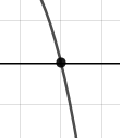
\includegraphics[width=0.3\textwidth]{../Figures/polyZeroBehaviorAB.png}
\end{center}\begin{enumerate}[label=\Alph*.]
\begin{multicols}{2}
\item 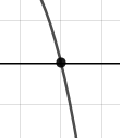
\includegraphics[width = 0.3\textwidth]{../Figures/polyZeroBehaviorAB.png}
\item 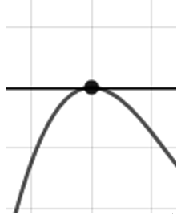
\includegraphics[width = 0.3\textwidth]{../Figures/polyZeroBehaviorBB.png}
\item 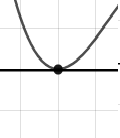
\includegraphics[width = 0.3\textwidth]{../Figures/polyZeroBehaviorCB.png}
\item 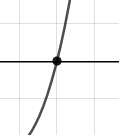
\includegraphics[width = 0.3\textwidth]{../Figures/polyZeroBehaviorDB.png}
\end{multicols}\item None of the above.\end{enumerate}
\textbf{General Comment:} You will need to sketch the entire graph, then zoom in on the zero the question asks about.
}
\litem{
Describe the end behavior of the polynomial below.
\[ f(x) = 8(x + 4)^{3}(x - 4)^{6}(x + 9)^{4}(x - 9)^{5} \]The solution is the graph below, which is option C.
\begin{center}
    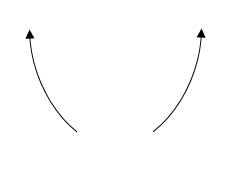
\includegraphics[width=0.3\textwidth]{../Figures/polyEndBehaviorCB.png}
\end{center}\begin{enumerate}[label=\Alph*.]
\begin{multicols}{2}
\item 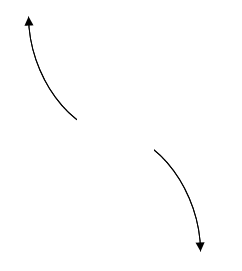
\includegraphics[width = 0.3\textwidth]{../Figures/polyEndBehaviorAB.png}
\item 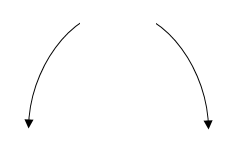
\includegraphics[width = 0.3\textwidth]{../Figures/polyEndBehaviorBB.png}
\item 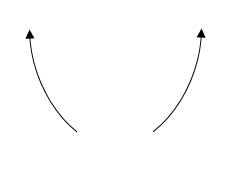
\includegraphics[width = 0.3\textwidth]{../Figures/polyEndBehaviorCB.png}
\item 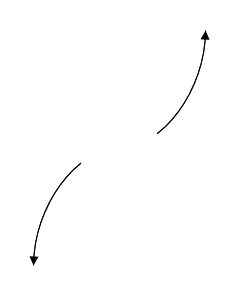
\includegraphics[width = 0.3\textwidth]{../Figures/polyEndBehaviorDB.png}
\end{multicols}\item None of the above.\end{enumerate}
\textbf{General Comment:} Remember that end behavior is determined by the leading coefficient AND whether the \textbf{sum} of the multiplicities is positive or negative.
}
\litem{
Describe the zero behavior of the zero $x = 4$ of the polynomial below.
\[ f(x) = 4(x + 2)^{5}(x - 2)^{4}(x + 4)^{5}(x - 4)^{4} \]The solution is the graph below, which is option C.
\begin{center}
    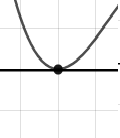
\includegraphics[width=0.3\textwidth]{../Figures/polyZeroBehaviorCopyCB.png}
\end{center}\begin{enumerate}[label=\Alph*.]
\begin{multicols}{2}
\item 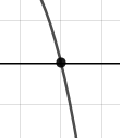
\includegraphics[width = 0.3\textwidth]{../Figures/polyZeroBehaviorCopyAB.png}
\item 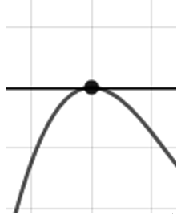
\includegraphics[width = 0.3\textwidth]{../Figures/polyZeroBehaviorCopyBB.png}
\item 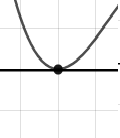
\includegraphics[width = 0.3\textwidth]{../Figures/polyZeroBehaviorCopyCB.png}
\item 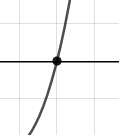
\includegraphics[width = 0.3\textwidth]{../Figures/polyZeroBehaviorCopyDB.png}
\end{multicols}\item None of the above.\end{enumerate}
\textbf{General Comment:} You will need to sketch the entire graph, then zoom in on the zero the question asks about.
}
\litem{
Describe the end behavior of the polynomial below.
\[ f(x) = 2(x + 3)^{4}(x - 3)^{9}(x + 9)^{4}(x - 9)^{5} \]The solution is the graph below, which is option C.
\begin{center}
    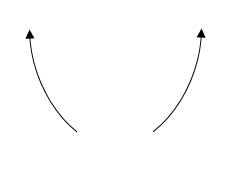
\includegraphics[width=0.3\textwidth]{../Figures/polyEndBehaviorCopyCB.png}
\end{center}\begin{enumerate}[label=\Alph*.]
\begin{multicols}{2}
\item 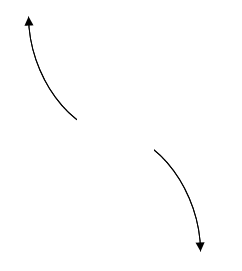
\includegraphics[width = 0.3\textwidth]{../Figures/polyEndBehaviorCopyAB.png}
\item 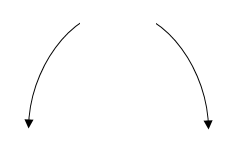
\includegraphics[width = 0.3\textwidth]{../Figures/polyEndBehaviorCopyBB.png}
\item 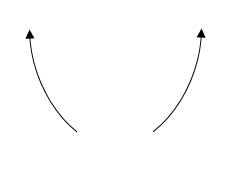
\includegraphics[width = 0.3\textwidth]{../Figures/polyEndBehaviorCopyCB.png}
\item 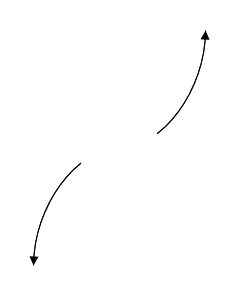
\includegraphics[width = 0.3\textwidth]{../Figures/polyEndBehaviorCopyDB.png}
\end{multicols}\item None of the above.\end{enumerate}
\textbf{General Comment:} Remember that end behavior is determined by the leading coefficient AND whether the \textbf{sum} of the multiplicities is positive or negative.
}
\litem{
Construct the lowest-degree polynomial given the zeros below. Then, choose the intervals that contain the coefficients of the polynomial in the form $x^3+bx^2+cx+d$.
\[ -4 - 5 i \text{ and } -4 \]The solution is \( x^{3} +12 x^{2} +73 x + 164 \), which is option A.\begin{enumerate}[label=\Alph*.]
\item \( b \in [6, 13], c \in [72.58, 73.76], \text{ and } d \in [162.4, 169] \)

* $x^{3} +12 x^{2} +73 x + 164$, which is the correct option.
\item \( b \in [-3, 10], c \in [8.81, 9.58], \text{ and } d \in [19.5, 21.2] \)

$x^{3} + x^{2} +9 x + 20$, which corresponds to multiplying out $(x + 5)(x + 4)$.
\item \( b \in [-3, 10], c \in [7.93, 8.59], \text{ and } d \in [15.7, 18.2] \)

$x^{3} + x^{2} +8 x + 16$, which corresponds to multiplying out $(x + 4)(x + 4)$.
\item \( b \in [-15, -4], c \in [72.58, 73.76], \text{ and } d \in [-165.5, -160.5] \)

$x^{3} -12 x^{2} +73 x -164$, which corresponds to multiplying out $(x-(-4 - 5 i))(x-(-4 + 5 i))(x -4)$.
\item \( \text{None of the above.} \)

This corresponds to making an unanticipated error or not understanding how to use nonreal complex numbers to create the lowest-degree polynomial. If you chose this and are not sure what you did wrong, please contact the coordinator for help.
\end{enumerate}

\textbf{General Comment:} Remember that the conjugate of $a+bi$ is $a-bi$. Since these zeros always come in pairs, we need to multiply out $(x-(-4 - 5 i))(x-(-4 + 5 i))(x-(-4))$.
}
\litem{
Construct the lowest-degree polynomial given the zeros below. Then, choose the intervals that contain the coefficients of the polynomial in the form $x^3+bx^2+cx+d$.
\[ -3 + 5 i \text{ and } -4 \]The solution is \( x^{3} +10 x^{2} +58 x + 136 \), which is option B.\begin{enumerate}[label=\Alph*.]
\item \( b \in [-12, -7], c \in [50, 59], \text{ and } d \in [-140, -131] \)

$x^{3} -10 x^{2} +58 x -136$, which corresponds to multiplying out $(x-(-3 + 5 i))(x-(-3 - 5 i))(x -4)$.
\item \( b \in [5, 18], c \in [50, 59], \text{ and } d \in [136, 142] \)

* $x^{3} +10 x^{2} +58 x + 136$, which is the correct option.
\item \( b \in [-3, 9], c \in [-5, 5], \text{ and } d \in [-26, -19] \)

$x^{3} + x^{2} -x -20$, which corresponds to multiplying out $(x -5)(x + 4)$.
\item \( b \in [-3, 9], c \in [2, 14], \text{ and } d \in [7, 17] \)

$x^{3} + x^{2} +7 x + 12$, which corresponds to multiplying out $(x + 3)(x + 4)$.
\item \( \text{None of the above.} \)

This corresponds to making an unanticipated error or not understanding how to use nonreal complex numbers to create the lowest-degree polynomial. If you chose this and are not sure what you did wrong, please contact the coordinator for help.
\end{enumerate}

\textbf{General Comment:} Remember that the conjugate of $a+bi$ is $a-bi$. Since these zeros always come in pairs, we need to multiply out $(x-(-3 + 5 i))(x-(-3 - 5 i))(x-(-4))$.
}
\litem{
Which of the following equations \textit{could} be of the graph presented below?

\begin{center}
    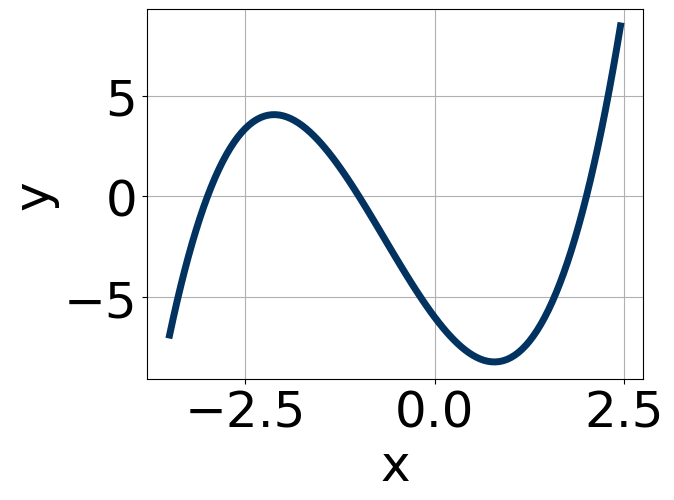
\includegraphics[width=0.5\textwidth]{../Figures/polyGraphToFunctionCopyB.png}
\end{center}


The solution is \( 13(x + 3)^{7} (x + 1)^{5} (x - 2)^{7} \), which is option E.\begin{enumerate}[label=\Alph*.]
\item \( 4(x + 3)^{4} (x + 1)^{4} (x - 2)^{11} \)

The factors $-3$ and $-1$ have have been odd power.
\item \( 18(x + 3)^{4} (x + 1)^{9} (x - 2)^{7} \)

The factor $-3$ should have been an odd power.
\item \( -15(x + 3)^{8} (x + 1)^{9} (x - 2)^{7} \)

The factor $(x + 3)$ should have an odd power and the leading coefficient should be the opposite sign.
\item \( -19(x + 3)^{7} (x + 1)^{5} (x - 2)^{11} \)

This corresponds to the leading coefficient being the opposite value than it should be.
\item \( 13(x + 3)^{7} (x + 1)^{5} (x - 2)^{7} \)

* This is the correct option.
\end{enumerate}

\textbf{General Comment:} General Comments: Draw the x-axis to determine which zeros are touching (and so have even multiplicity) or cross (and have odd multiplicity).
}
\litem{
Construct the lowest-degree polynomial given the zeros below. Then, choose the intervals that contain the coefficients of the polynomial in the form $ax^3+bx^2+cx+d$.
\[ \frac{-7}{5}, \frac{-5}{3}, \text{ and } \frac{3}{4} \]The solution is \( 60x^{3} +139 x^{2} +2 x -105 \), which is option A.\begin{enumerate}[label=\Alph*.]
\item \( a \in [60, 61], b \in [135, 149], c \in [-4, 9], \text{ and } d \in [-115, -100] \)

* $60x^{3} +139 x^{2} +2 x -105$, which is the correct option.
\item \( a \in [60, 61], b \in [-229, -223], c \in [275, 281], \text{ and } d \in [-115, -100] \)

$60x^{3} -229 x^{2} +278 x -105$, which corresponds to multiplying out $(5x -7)(3x -5)(4x -3)$.
\item \( a \in [60, 61], b \in [135, 149], c \in [-4, 9], \text{ and } d \in [104, 108] \)

$60x^{3} +139 x^{2} +2 x + 105$, which corresponds to multiplying everything correctly except the constant term.
\item \( a \in [60, 61], b \in [-32, -25], c \in [-153, -151], \text{ and } d \in [104, 108] \)

$60x^{3} -29 x^{2} -152 x + 105$, which corresponds to multiplying out $(5x -7)(3x + 5)(4x -3)$.
\item \( a \in [60, 61], b \in [-142, -136], c \in [-4, 9], \text{ and } d \in [104, 108] \)

$60x^{3} -139 x^{2} +2 x + 105$, which corresponds to multiplying out $(5x -7)(3x -5)(4x + 3)$.
\end{enumerate}

\textbf{General Comment:} To construct the lowest-degree polynomial, you want to multiply out $(5x + 7)(3x + 5)(4x -3)$
}
\litem{
Which of the following equations \textit{could} be of the graph presented below?

\begin{center}
    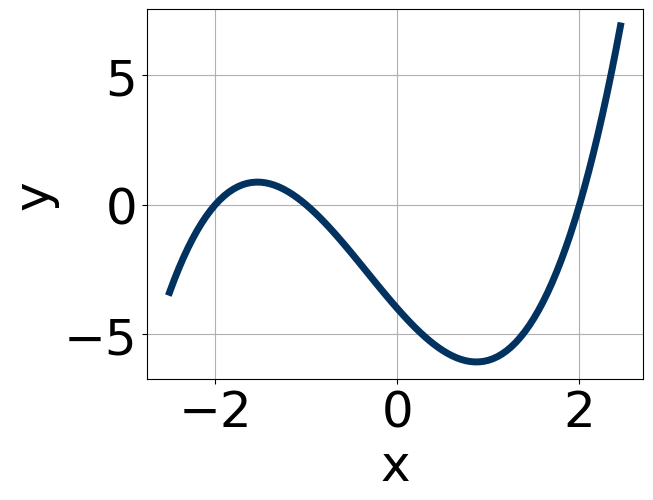
\includegraphics[width=0.5\textwidth]{../Figures/polyGraphToFunctionB.png}
\end{center}


The solution is \( 8(x + 2)^{7} (x - 2)^{9} (x + 1)^{7} \), which is option B.\begin{enumerate}[label=\Alph*.]
\item \( -5(x + 2)^{4} (x - 2)^{5} (x + 1)^{5} \)

The factor $(x + 2)$ should have an odd power and the leading coefficient should be the opposite sign.
\item \( 8(x + 2)^{7} (x - 2)^{9} (x + 1)^{7} \)

* This is the correct option.
\item \( 17(x + 2)^{4} (x - 2)^{10} (x + 1)^{11} \)

The factors $-2$ and $2$ have have been odd power.
\item \( 18(x + 2)^{8} (x - 2)^{9} (x + 1)^{9} \)

The factor $-2$ should have been an odd power.
\item \( -16(x + 2)^{7} (x - 2)^{11} (x + 1)^{7} \)

This corresponds to the leading coefficient being the opposite value than it should be.
\end{enumerate}

\textbf{General Comment:} General Comments: Draw the x-axis to determine which zeros are touching (and so have even multiplicity) or cross (and have odd multiplicity).
}
\end{enumerate}

\end{document}